\documentclass[11pt,a4paper]{article}
\usepackage{amsmath,amssymb,amsthm}
% algorithm/algpseudocode: uncomment when compiling locally
% \usepackage{algorithm}
% \usepackage{algpseudocode}
\usepackage{float}  % for [H] placement as fallback
\usepackage{graphicx}
\usepackage{booktabs}
\usepackage{tikz}
\usetikzlibrary{bayesnet,arrows.meta,positioning}
\usepackage{hyperref}
\usepackage{cleveref}

% Theorem environments
\newtheorem{definition}{Definition}
\newtheorem{theorem}{Theorem}
\newtheorem{lemma}{Lemma}
\newtheorem{proposition}{Proposition}
\newtheorem{corollary}{Corollary}
\newtheorem{remark}{Remark}

% Custom commands
\DeclareMathOperator{\Cat}{Cat}
\DeclareMathOperator{\Ber}{Ber}
\DeclareMathOperator{\supp}{supp}
\newcommand{\E}{\mathbb{E}}
\newcommand{\Prob}{\mathbb{P}}
\newcommand{\cA}{\mathcal{A}}
\newcommand{\cB}{\mathcal{B}}
\newcommand{\cS}{\mathcal{S}}
\newcommand{\cT}{\mathcal{T}}
\newcommand{\cN}{\mathcal{N}}
\newcommand{\cP}{\mathcal{P}}
\newcommand{\cE}{\mathcal{E}}

\title{Learning ZX-Calculus Simplification with Generative Flow Networks}
\author{
Joseph Denman \\
% affiliation
}
\date{\today}

\begin{document}

\maketitle

\begin{abstract}
We present AlphaZX, a system that learns to simplify quantum circuits
expressed in the ZX-calculus using Generative Flow Networks (GFlowNets).
Unlike reinforcement learning approaches that converge to a single
policy, GFlowNets learn to sample diverse simplification trajectories
with probability proportional to their quality, producing a distribution
over effective strategies rather than a single fixed procedure.  AlphaZX
operates on a provably complete four-rule system for the Clifford+T
fragment---spider fusion, local complementation, pivoting, and
gadgetization---requiring no hand-crafted simplification heuristics.  To
handle the combinatorially large, variable-structure action space of ZX
rewrites, we introduce a hierarchical action distribution that factorizes
each rewrite into conditional sub-decisions, each becoming an explicit
transition in the GFlowNet's flow DAG for fine-grained credit assignment.
We describe the training methodology---including sub-trajectory balance
for long-horizon credit assignment, reward exponent annealing, and
diversity-aware replay---and evaluate the system against PyZX on random
Clifford+T circuits.
% TODO: Add summary of key experimental results once available.
\end{abstract}


% ======================================================================
\section{Introduction}\label{sec:intro}
% ======================================================================

Reducing the non-Clifford gate count of quantum circuits is a central
problem in both near-term and fault-tolerant quantum computing.  T-gates
(and more generally, non-Clifford rotations) dominate the cost of
fault-tolerant implementations via magic state
distillation~\cite{bravyi2005universal}, so even modest T-count
reductions translate directly into lower overhead.

The ZX-calculus~\cite{coecke2011interacting} provides a graphical
language for reasoning about quantum circuits in which circuit identities
become local graph rewriting rules.  Tools such as
PyZX~\cite{kissinger2020pyzx} exploit this framework to achieve
state-of-the-art T-count optimization through carefully engineered
simplification pipelines.  However, these pipelines apply a fixed
sequence of heuristic passes, leaving open the question of whether
learned strategies could discover simplifications that hand-crafted
orderings miss.

Recent work has applied reinforcement learning (RL) to this problem.
Riu et al.~\cite{riu2025rl} train a PPO agent with a graph neural
network (GNN) policy to select ZX-calculus rewrites, achieving strong
generalization from small training circuits to much larger ones.  Their
approach demonstrates that learned policies can match or exceed
heuristic baselines.  However, RL methods converge to a single
deterministic (or near-deterministic) policy, which may miss alternative
simplification pathways.

We take a different approach.  Generative Flow Networks
(GFlowNets)~\cite{bengio2021flow} are a framework for training
stochastic policies that sample composite objects---here, simplification
trajectories---with probability proportional to a reward function.
Rather than converging to the single best trajectory, a GFlowNet learns
to distribute probability mass across \emph{all} high-reward
trajectories in proportion to their quality.  This diversity property is
well suited to ZX-calculus simplification, where many distinct rewrite
sequences can achieve similar T-count reductions, and where maintaining a
portfolio of strategies may be valuable for downstream tasks such as
hardware-aware compilation.

Applying GFlowNets to ZX-calculus simplification raises three technical
challenges that this paper addresses:

\begin{enumerate}
\item \textbf{Structured, variable-size action space.}  Each rewrite
action comprises a rule type, a target node, and (for some rules) a
phase, new edges, and edge transfers.  The joint space is combinatorially
large and varies in structure across rule types.  We introduce the
\emph{AlphaZX distribution}, a hierarchical factorization that decomposes
each action into conditional sub-decisions while maintaining exact
log-likelihood computation and differentiability
(\cref{sec:distribution}).

\item \textbf{Long credit-assignment horizon.}  Each rewrite decomposes
into 2--5 sub-decisions, and trajectories span 10--20 rewrites, yielding
40--70 sub-transitions per trajectory.  We make each sub-decision an
explicit transition in the GFlowNet DAG, and adopt the sub-trajectory
balance (SubTB) loss~\cite{madan2023subtb} to provide dense learning
signals across this long horizon (\cref{sec:subactions,sec:subtb}).

\item \textbf{Sparse rewards in early training.}  With a random policy,
almost no trajectory achieves meaningful T-gate reduction, causing the
reward landscape to collapse to a constant floor.  We address this
through reward exponent annealing, intermediate reward shaping, and
diversity-aware prioritized replay (\cref{sec:training}).
\end{enumerate}

AlphaZX operates on the four-rule system of spider fusion, local
complementation, pivoting, and gadgetization, which is provably complete
for the Clifford+T fragment~\cite{jeandel2018complete,
backens2021completeness}.  Completeness ensures that any simplification
achievable by any ZX-calculus strategy lies within the agent's search
space.


% ======================================================================
\section{Background}\label{sec:background}
% ======================================================================

\subsection{ZX-Calculus}\label{sec:bg_zx}

The ZX-calculus~\cite{coecke2011interacting} is a graphical language for
quantum computation.  A ZX diagram is an open graph whose vertices
(\emph{spiders}) are labelled by a basis (Z~or~X) and a phase
$\phi \in [0, 2\pi)$, and whose edges represent qubit wires.  Boundary
vertices mark circuit inputs and outputs.  Any quantum circuit over the
Clifford+T gate set can be translated into a ZX diagram, and conversely
any ZX diagram satisfying certain connectivity constraints corresponds to
a quantum circuit~\cite{backens2021completeness}.

\paragraph{Rewrite rules.}
Equalities between quantum circuits correspond to local rewriting rules
on ZX diagrams.  We use the four-rule system consisting of spider fusion
(F), local complementation (B), pivoting (Y), and gadgetization
(F-Right), following Backens et al.~\cite{backens2021completeness}.  Each
rule has Z- and X-basis variants and left/right orientations, yielding 10
concrete action types (\cref{tab:action_types}).  Jeandel, Perdrix, and
Vilmart~\cite{jeandel2018complete} established that this rule set is
\emph{complete} for the Clifford+T fragment: any equality between
Clifford+T circuits that holds in the standard interpretation can be
derived using only these rules.


\subsection{Generative Flow Networks}\label{sec:bg_gflownet}

A GFlowNet~\cite{bengio2021flow} learns a stochastic policy that
constructs objects through a sequence of actions in a directed acyclic
graph (DAG) of states, such that the probability of generating an object
$x$ is proportional to a given reward $R(x) \ge 0$.  Formally, given a
DAG with initial state $s_0$ and terminal states, a GFlowNet defines a
forward policy $P_F(a \mid s)$ and a backward policy $P_B(a \mid s')$
satisfying the \emph{trajectory balance} condition~\cite{malkin2022trajectory}:
\begin{equation}\label{eq:tb_bg}
Z \prod_{i=1}^{N} P_F(a_i \mid s_{i-1})
= R(s_N) \prod_{i=1}^{N} P_B(a_i \mid s_i),
\end{equation}
where $Z$ is a learnable partition function and $(s_0, a_1, s_1, \ldots,
a_N, s_N)$ is a complete trajectory.  Training minimizes the squared
log-ratio of the two sides of~\cref{eq:tb_bg}, encouraging the forward
policy to sample trajectories reaching terminal state~$x$ with
probability $P(\tau \to x) \propto R(x)$.

The \emph{sub-trajectory balance} (SubTB)
extension~\cite{madan2023subtb} applies the flow-conservation constraint
to all contiguous sub-sequences, not just complete trajectories,
providing denser learning signals for long-horizon problems.


% ======================================================================
\section{Method}\label{sec:method}
% ======================================================================

We formulate ZX-calculus simplification as a sequential decision process
over a DAG of states and train a GFlowNet to sample simplification
trajectories with probability proportional to their quality.  This
section describes the state representation (\cref{sec:states}), the
hierarchical action distribution (\cref{sec:distribution}), the
decomposed sub-action architecture (\cref{sec:subactions}), the graph
neural network backbone (\cref{sec:architecture}), and the training
procedure (\cref{sec:training}).


% ----------------------------------------------------------------------
\subsection{ZX Diagrams as GFlowNet States}\label{sec:states}
% ----------------------------------------------------------------------

\paragraph{Match diagram.}
Rather than feeding the raw ZX graph to the policy network, we construct
a \emph{match diagram}: a directed graph whose vertices are all currently
applicable rewrite-rule matches.  Each match node records the rule type,
the phase of the matched spider, and the set of ZX vertices it covers.
Edges connect matches that share underlying ZX vertices, encoding
structural dependencies between candidate rewrites.  This representation
scales with the number of available actions rather than with the raw
diagram size, and provides an inductive bias for the GNN to reason about
which rewrites interact.

\begin{table}[t]
\centering
\caption{Action types in the AlphaZX rewrite system.  F-Right actions
require five sequential sub-decisions (type, node, phase, new edge,
transfer edges); all others require two (type, node).}
\label{tab:action_types}
\small
\begin{tabular}{clll}
\toprule
Index & Name & Rule & Sub-decisions \\
\midrule
0 & \texttt{f-right-z} & Gadgetization (Z) & 5 \\
1 & \texttt{f-right-x} & Gadgetization (X) & 5 \\
2 & \texttt{f-left-z}  & Spider fusion (Z) & 2 \\
3 & \texttt{f-left-x}  & Spider fusion (X) & 2 \\
4 & \texttt{b-right}   & Local complementation ($\to$) & 2 \\
5 & \texttt{b-left}    & Local complementation ($\leftarrow$) & 2 \\
6 & \texttt{y-right-z} & Pivoting (Z, $\to$) & 2 \\
7 & \texttt{y-left-z}  & Pivoting (Z, $\leftarrow$) & 2 \\
8 & \texttt{y-right-x} & Pivoting (X, $\to$) & 2 \\
9 & \texttt{y-left-x}  & Pivoting (X, $\leftarrow$) & 2 \\
\bottomrule
\end{tabular}
\end{table}

\paragraph{State space and reward.}
A GFlowNet state $s \in \cS$ is a ZX diagram together with its match
diagram and the corresponding \textsc{PyTorch Geometric} graph object.  A
trajectory $\tau = (s_0, a_0, s_1, \ldots, s_T)$ is a sequence of states
connected by rewrite actions, where $s_0$ is the initial circuit and
$s_T$ is the terminal state (either no non-Clifford gates remain or no
further rewrites are applicable).  The terminal reward is
\begin{equation}\label{eq:reward}
R(s_T) = \max\!\bigl(\epsilon,\;
    r(s_T)^{\beta}\bigr),
\qquad
r(s_T) = \frac{T_{\mathrm{init}} - T_{\mathrm{final}}}{T_{\mathrm{init}}},
\end{equation}
where $T_{\mathrm{init}}$ and $T_{\mathrm{final}}$ are the initial and
final T-gate counts, $\beta$ is a sharpness exponent, and $\epsilon$ is a
small floor preventing $\log R = -\infty$ in the loss.


% ----------------------------------------------------------------------
\subsection{The AlphaZX Distribution}\label{sec:distribution}
% ----------------------------------------------------------------------

Each rewrite action $a = (t, n, \phi, e_{\mathrm{new}},
e_{\mathrm{tr}})$ specifies a rule type~$t$, a target node~$n$, a
phase~$\phi$, a new-edge count~$e_{\mathrm{new}}$, and a binary vector
of edge transfers~$e_{\mathrm{tr}}$.  The joint space~$\cA$ is
combinatorially large: even a modest diagram with 50 match nodes and 8
possible phases has $|\cA| > 10^6$ when all five components are free.

We define a hierarchical factorization that mirrors the logical structure
of graph rewriting:

\begin{definition}[AlphaZX Distribution]\label{def:alphazx_dist}
Given state $s \in \cS$, the AlphaZX distribution $\pi(\cdot \mid s)$
over actions is:
\begin{align}\label{eq:factorization}
\pi(a \mid s) &= \pi_t(t \mid s)\;
               \pi_n(n \mid t, s)\;
               \pi_\phi(\phi \mid t, n, s) \notag \\
            &\quad\; \pi_e(e_{\mathrm{new}} \mid t, n, s)\;
               \pi_{\mathrm{tr}}(e_{\mathrm{tr}} \mid t, n, s).
\end{align}
\end{definition}

\noindent
This factorization induces a directed graphical model over the action
components:

\begin{center}
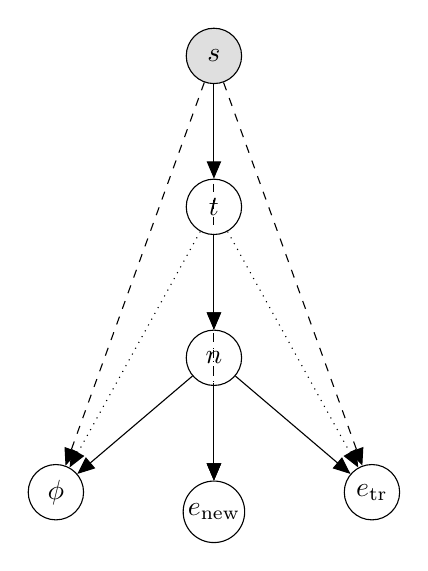
\begin{tikzpicture}
  \node[obs] (s) {$s$};%
  \node[latent, below=1.2 of s] (t) {$t$};%
  \node[latent, below=1.2 of t] (n) {$n$};%
  \node[latent, below left=1.2 and 1.5 of n] (phi) {$\phi$};%
  \node[latent, below=1.2 of n] (new) {$e_{\text{new}}$};%
  \node[latent, below right=1.2 and 1.5 of n] (trans) {$e_{\text{tr}}$};%
  \edge{s}{t}
  \edge{t}{n}
  \edge{n}{phi,new,trans}
  \edge[dashed]{s}{n,phi,new,trans}
  \edge[dotted]{t}{phi,new,trans}
\end{tikzpicture}
\end{center}

The first factor selects a rule type via a masked categorical over the
types with at least one applicable match.  The second selects a node,
masked to the nodes valid for the chosen type.  The remaining three
factors are \emph{type-conditional}: for non-F-Right rules (types 2--9),
$\phi$, $e_{\mathrm{new}}$, and $e_{\mathrm{tr}}$ collapse to point
masses, since these rules require no additional parameters.

\paragraph{Component distributions.}
Each factor has a specific parametric form:
\begin{enumerate}
\item \textbf{Type selection.}
$\pi_t(t \mid s) = \Cat(t;\, \theta_t(s))$, where
$\theta_t(s) \in \Delta^{|\cT|-1}$ is produced by the policy network and
masked to types with available matches.

\item \textbf{Node selection.}
$\pi_n(n \mid t,s) = \Cat(n;\, \theta_n(t,s))$, supported on
$\cN(t,s)$, the nodes valid for type~$t$.  Masking is implemented by
setting logits of invalid nodes to $-\infty$ before softmax:
\[
\tilde{f}_n(n,s,t) = \begin{cases}
f_n(n,s) & \text{if } n \in \cN(t,s) \\
-\infty & \text{otherwise,}
\end{cases}
\]
where $f_n$ is the neural network's node logit function.

\item \textbf{Phase selection.}
\[
\pi_\phi(\phi \mid t,n,s) = \begin{cases}
\Cat(\phi;\, \theta_\phi(t,n,s)) & \text{if } t \in \cT_{\text{F-Right}} \\
\delta_0(\phi) & \text{otherwise.}
\end{cases}
\]

\item \textbf{New edge count.}
\[
\pi_e(e_{\mathrm{new}} \mid t,n,s) = \begin{cases}
\Cat(e_{\mathrm{new}};\, \theta_e(t,n,s)) & \text{if } t \in \cT_{\text{F-Right}} \\
\delta_0(e_{\mathrm{new}}) & \text{otherwise.}
\end{cases}
\]

\item \textbf{Edge transfer.}
\[
\pi_{\mathrm{tr}}(e_{\mathrm{tr}} \mid t,n,s) = \begin{cases}
\prod_{i} \Ber(e_{\mathrm{tr},i};\, \sigma_i(t,n,s)) & \text{if } t \in \cT_{\text{F-Right}} \\
\delta_\emptyset(e_{\mathrm{tr}}) & \text{otherwise,}
\end{cases}
\]
where $\sigma_i$ are per-edge sigmoid outputs.
\end{enumerate}

The point masses for unused components ensure the joint remains a valid
probability distribution regardless of the chosen rule type: each such
factor contributes exactly~1 to the product in~\cref{eq:factorization}.

\paragraph{Properties.}
This design provides three properties important for GFlowNet training.
First, \emph{exact log-likelihood}: $\log \pi(a \mid s)$ decomposes as a
sum of component log-probabilities, each computable in $O(1)$ or
$O(|E_{\mathrm{eligible}}|)$ time---compared to $O(|\cA|)$ for a flat
categorical over the product space.  Second, \emph{differentiability}:
the masked softmax and Bernoulli log-probabilities are differentiable
with respect to the network parameters, enabling gradient-based GFlowNet
training.  Third, \emph{variable support}: invalid actions are excluded
by construction, so the policy never proposes illegal rewrites regardless
of the learned flow values.

\begin{proposition}[Consistency]\label{prop:consistency}
The AlphaZX distribution defines a valid probability measure:
$\sum_{a \in \cA} \pi(a \mid s) = 1$ for all $s \in \cS$.
\end{proposition}
\begin{proof}
By the chain rule and the normalization of each component (including
point masses):
$\sum_a \pi(a \mid s)
= \sum_t \pi_t(t \mid s)
  \sum_n \pi_n(n \mid t,s)
  \sum_\phi \pi_\phi(\phi \mid t,n,s)
  \sum_{e_{\mathrm{new}}} \pi_e(e_{\mathrm{new}} \mid t,n,s)
  \sum_{e_{\mathrm{tr}}} \pi_{\mathrm{tr}}(e_{\mathrm{tr}} \mid t,n,s)
= \sum_t \pi_t(t \mid s) \cdot 1 \cdot 1 \cdot 1 \cdot 1 = 1$.
\end{proof}


% ----------------------------------------------------------------------
\subsection{Decomposed Sub-Action GFlowNet}\label{sec:subactions}
% ----------------------------------------------------------------------

Standard GFlowNet formulations treat each action as an atomic transition.
In our setting, this would mean the flow equations assign credit to an
entire composite action as a single decision.  When trajectories span
10--20 rewrites and each F-Right rewrite involves 5 sub-decisions, the
resulting credit-assignment problem covers 40--70 effective decision
points, well beyond the horizon where trajectory balance provides
efficient learning~\cite{malkin2022trajectory}.

We instead \emph{decompose} each rewrite into its constituent
sub-decisions, making each one an explicit transition in the GFlowNet's
DAG.  A single rewrite of type~$t$ applied to node~$n$ becomes the
sub-transition sequence:
\begin{equation}\label{eq:subactions}
s \xrightarrow{\text{type } t} s'_1
  \xrightarrow{\text{node } n} s'_2
  \xrightarrow{\text{phase}} s'_3
  \xrightarrow{\text{edge}} s'_4
  \xrightarrow{\text{transfer}} s_{k+1},
\end{equation}
where $s'_1, \ldots, s'_4$ are \emph{partial-action states} (the diagram
has not yet changed) and $s_{k+1}$ is the new ZX diagram after the
rewrite is applied.  Non-F-Right rewrites produce only two
sub-transitions (type and node).

Each sub-transition carries its own forward log-probability $\log P_F$
from the corresponding component of the AlphaZX distribution
(\cref{def:alphazx_dist}), and its own backward log-probability
$\log P_B$ from a uniform backward policy over valid choices at that
sub-step.  The trajectory balance condition then becomes:
\begin{equation}\label{eq:tb}
\log Z + \sum_{i=1}^{N} \log P_F(a_i \mid s_{i-1})
= \log R(s_T) + \sum_{i=1}^{N} \log P_B(a_i \mid s_i),
\end{equation}
where $N$ is the total number of \emph{sub-transitions} (not the number
of rewrites).  This decomposition gives the loss gradient direct access
to each sub-decision's probability, enabling fine-grained credit
assignment without requiring intermediate rewards for sub-steps within a
single rewrite.

The full sampling procedure is summarized in \cref{alg:sampling}.

% Algorithm 1 (requires algorithm + algpseudocode packages for local build)
\begin{figure}[t]
\centering
\fbox{\parbox{0.92\columnwidth}{%
\textbf{Algorithm 1:} Sampling one rewrite step (decomposed sub-actions)
\label{alg:sampling}
\smallskip\hrule\smallskip
\textbf{Input:} State $s$, policy network $\theta$ \\[2pt]
1.\quad Compute distribution $\pi(\cdot \mid s)$ via forward pass \\
2.\quad $t \sim \Cat(\theta_t(s))$ \hfill [masked to available types] \\
3.\quad $n \sim \Cat(\theta_n(t,s))$ \hfill [masked to valid nodes for $t$] \\
4.\quad \textbf{if} $t \in \cT_{\text{F-Right}}$ \textbf{then} \\
5.\qquad $\phi \sim \Cat(\theta_\phi(t,n,s))$ \\
6.\qquad $e_{\mathrm{new}} \sim \Cat(\theta_e(t,n,s))$ \\
7.\qquad $e_{\mathrm{tr}} \sim \prod_i \Ber(\sigma_i(t,n,s))$ \\
8.\quad \textbf{else} \\
9.\qquad $\phi \gets 0$;\; $e_{\mathrm{new}} \gets 0$;\; $e_{\mathrm{tr}} \gets \emptyset$ \\
10.\;\; Apply rewrite $(t, n, \phi, e_{\mathrm{new}}, e_{\mathrm{tr}})$ to $s$ \\
11.\;\; \textbf{Return} new state $s'$, sub-transition log-probabilities
}}
\end{figure}


% ----------------------------------------------------------------------
\subsection{Network Architecture}\label{sec:architecture}
% ----------------------------------------------------------------------

The policy and value functions share a Graph Positional Transformer (GPS)
backbone~\cite{rampavsek2022recipe} operating on the match-diagram graph.

\paragraph{Input features.}
Each match-diagram node is embedded as the concatenation of a learned
node-type embedding (over the 10 action types plus boundary nodes), a
sinusoidal phase encoding, and a random-walk positional
encoding~\cite{dwivedi2022graph} that captures structural position in the
match graph.  Edge features encode the relationship type between matches
(shared node, adjacency, etc.).

\paragraph{GPS layers.}
The backbone consists of $L$ GPS layers (default $L{=}4$), each combining
a \textsc{ResGatedGraphConv} message-passing step with multi-head
self-attention ($H{=}4$ heads), followed by a two-layer MLP with residual
connections.  This hybrid architecture captures both local graph structure
through message passing and long-range dependencies through attention.

\paragraph{Output heads.}
The GPS output feeds two heads:
\begin{itemize}
\item A \emph{policy head} producing the five distribution components of
\cref{eq:factorization}: a \textsc{RewriteTypeSelector} (global
pooling $\to$ 10-way softmax), a \textsc{NodeSelector} (per-node logits
masked by type), and type-conditional \textsc{PhaseSelector},
\textsc{NewEdgeSelector}, and \textsc{TransferEdgeSelector} heads (each
a small MLP from the selected node's embedding).
\item A \emph{value head} (global pooling $\to$ scalar) producing a
state-flow estimate $\log \hat{F}(s)$, used by the sub-trajectory
balance loss (\cref{sec:subtb}).
\end{itemize}
All parameters are trained jointly.  A separate learnable scalar $\log Z$
serves as the partition-function estimate for the trajectory balance
objective.


% ----------------------------------------------------------------------
\subsection{Training}\label{sec:training}
% ----------------------------------------------------------------------

Training a GFlowNet over long trajectories with sparse terminal rewards
presents several challenges: reward sparsity in early training, long
credit-assignment chains, and mode collapse onto deterministic
trajectories.  We address each with a targeted mechanism.

\subsubsection{Sub-Trajectory Balance}\label{sec:subtb}

Trajectory balance (\cref{eq:tb}) provides a single scalar constraint per
trajectory.  For trajectories with 40--70 sub-transitions, this global
signal is too diffuse for efficient learning.  We adopt the SubTB
objective of Madan et al.~\cite{madan2023subtb}, which enforces flow
conservation over all contiguous sub-sequences of rewrites.

Let $n$ denote the number of rewrites in a trajectory, and let
$\hat{F}(s_k)$ be the value head's flow estimate at the state before
rewrite~$k$.  Define $\hat{F}(s_0) = Z$ and
$\hat{F}(s_n) = R(s_T)$.  The SubTB($\lambda$) loss is
\begin{equation}\label{eq:subtb}
\mathcal{L}_{\mathrm{SubTB}} = \frac{1}{W}
\sum_{0 \le i < j \le n}
\lambda^{j-i-1}\,\delta_{ij}^2,
\end{equation}
where $W = \sum_{i<j} \lambda^{j-i-1}$ is a normalizing constant and
\begin{equation}\label{eq:subtb_delta}
\delta_{ij} = \log \hat{F}(s_i)
  + \sum_{k=i}^{j-1} \log P_F^{(k)}
  - \log \hat{F}(s_j)
  - \sum_{k=i}^{j-1} \log P_B^{(k)},
\end{equation}
with $\log P_F^{(k)}$ and $\log P_B^{(k)}$ denoting the total forward
and backward log-probabilities over all sub-transitions of rewrite~$k$.
The parameter $\lambda \in [0,1]$ interpolates between detailed balance
($\lambda{=}0$) and full trajectory balance ($\lambda{=}1$).  We use
$\lambda{=}0.9$.

Sub-trajectory windows are defined at the \emph{rewrite} level, not the
sub-transition level, because intermediate flow estimates $\hat{F}(s_k)$
are meaningful only at rewrite boundaries (actual ZX diagram states), not
at partial-action states within a rewrite.  The per-rewrite forward and
backward probabilities are computed by summing sub-transition
log-probabilities within each rewrite, leveraging the decomposed
architecture of \cref{sec:subactions}.

\subsubsection{Reward Exponent Annealing}\label{sec:annealing}

The reward function (\cref{eq:reward}) with high exponent $\beta$
concentrates probability mass on the best trajectories, which is
desirable at convergence but counterproductive early in training: when the
policy is random, almost no trajectory achieves a meaningful T-gate
reduction, and nearly all rewards collapse to the floor $\epsilon$.  We
anneal the exponent linearly from $\beta_0 = 1$ to $\beta_{\max} = 4$
over the first $W$ training iterations:
\begin{equation}\label{eq:anneal}
\beta(t) = \beta_0 + (\beta_{\max} - \beta_0)
    \cdot \min\!\Bigl(1,\; \frac{t}{W}\Bigr).
\end{equation}
With $\beta{=}1$, the reward is simply the reduction ratio $r(s_T)$,
which is non-trivial for any trajectory that removes even a single
T-gate.  As training progresses, the sharpening exponent increasingly
concentrates flow on the highest-quality trajectories.

\subsubsection{Intermediate Reward Shaping}\label{sec:shaping}

Even with exponent annealing, the terminal reward provides no signal
about \emph{which rewrites within a trajectory} were productive.
Inspired by the GAFN framework~\cite{pan2023gafn}, we augment the
terminal reward with a multiplicative shaping bonus:
\begin{equation}\label{eq:shaping}
R_{\mathrm{shaped}} = R(s_T) \cdot
\exp\!\Biggl(\alpha \cdot
\frac{\sum_{k=1}^{n} \max(0,\;\Delta T_k)}{T_{\mathrm{init}}}
\Biggr),
\end{equation}
where $\Delta T_k = T_{k-1} - T_k$ is the T-gate change at rewrite~$k$
and $\alpha \ge 0$ is a shaping coefficient.  The $\max(0, \cdot)$
prevents telescoping: only positive reductions contribute, discriminating
trajectories with productive intermediate steps from those where no
individual rewrite helped.

\subsubsection{Prioritized Replay with Diversity}\label{sec:replay}

On-policy GFlowNet training discards trajectories after a single gradient
step.  We maintain a prioritized replay buffer that stores high-reward
trajectories and re-evaluates them under the current policy via
teacher-forced rollouts.  To prevent collapse to a single trajectory,
each entry~$e$ receives a diversity-aware priority:
\begin{equation}\label{eq:priority}
\mathrm{priority}(e) = R(e) + \gamma \cdot
\frac{1}{|\{e' \in \cB : \mathrm{fp}(e') = \mathrm{fp}(e)\}|},
\end{equation}
where $\mathrm{fp}(e)$ is the action-type fingerprint (the sequence of
rule types used) and $\gamma$ weights the diversity bonus.

\subsubsection{Optimization Details}\label{sec:optim}

We use Adam with a model learning rate of $10^{-3}$ and a separate
learning rate of $5 \times 10^{-2}$ for $\log Z$, following the standard
practice of using a higher rate for the scalar partition
function~\cite{malkin2022trajectory}.  The learning rate follows a cosine
schedule with warm restarts every 50 iterations.  Gradients are clipped
to a maximum norm of~10.  Each training iteration samples a batch of 64
trajectories, with a configurable fraction drawn from the replay buffer.


% ======================================================================
\section{Experiments}\label{sec:experiments}
% ======================================================================

% TODO: Fill in with experimental results.
% Planned subsections:
% 4.1 Setup (circuit generation, metrics, PyZX baseline)
% 4.2 Main results (T-count reduction, win/tie/loss vs PyZX)
% 4.3 Ablation studies (reward shaping, SubTB vs TB, annealing, replay)
% 4.4 Analysis of learned strategies (diversity, action distributions)


% ======================================================================
\section{Related Work}\label{sec:related}
% ======================================================================

\paragraph{ZX-calculus simplification.}
Kissinger and van de Wetering~\cite{kissinger2020pyzx} developed PyZX,
implementing heuristic simplification passes based on local
complementation and pivoting for Clifford circuit optimization.  Riu et
al.~\cite{riu2025rl} applied PPO with a GNN policy to learn ZX-diagram
rewrite strategies, achieving strong generalization from 5-qubit training
circuits to 80+ qubits.  Our work differs in using GFlowNets rather than
RL, which provides diverse trajectory sampling rather than convergence to
a single policy, and in operating on a minimal complete rule set rather
than PyZX's heuristic passes.

\paragraph{GFlowNets.}
Bengio et al.~\cite{bengio2021flow} introduced GFlowNets for
non-iterative diverse candidate generation.  Malkin et
al.~\cite{malkin2022trajectory} proposed trajectory balance for improved
credit assignment, and Madan et al.~\cite{madan2023subtb} extended this
with sub-trajectory balance for long-horizon problems.  GFlowNets have
been applied to molecular design~\cite{bengio2021flow}, combinatorial
optimization over graphs~\cite{zhang2023gflownet_combinatorial}, and DAG
generation.  To our knowledge, this is the first application of GFlowNets
to quantum circuit optimization.

\paragraph{ML for quantum compilation.}
Beyond ZX-calculus, reinforcement learning has been applied to quantum
circuit synthesis~\cite{fosel2021quantum}, fault-tolerant state
preparation, and adaptive selection of optimization
passes~\cite{mills2025adaptive}.  Diffusion models have been explored for
circuit synthesis.  These approaches typically operate at the gate level
rather than through a diagrammatic calculus.

\paragraph{Structured action spaces.}
The AlphaZX distribution is an instance of autoregressive factorization
over a structured action space, a technique used in complex game-playing
agents (e.g., the action space decomposition in
AlphaStar~\cite{vinyals2019grandmaster}) and structured prediction.  Our
contribution is the specific design for variable-structure ZX rewrites
and its integration with GFlowNet flow equations, where each factor
becomes an explicit sub-transition in the flow DAG.


% ======================================================================
\section{Conclusion}\label{sec:conclusion}
% ======================================================================

% TODO: Fill in once experimental results are available.
% Key points:
% - GFlowNets can learn ZX-calculus simplification from scratch
% - Decomposed sub-action design enables fine-grained credit assignment
% - Complete rule set ensures theoretical coverage
% - Diversity property is unique vs RL approaches
% - Limitations: computational cost, not yet beating PyZX
% - Future: scaling, transfer learning, hardware-aware compilation


% ======================================================================
% References
% ======================================================================

\bibliographystyle{plain}
% \bibliography{references}  % Uncomment when .bib file is ready

\begin{thebibliography}{99}

\bibitem{backens2021completeness}
M.~Backens, H.~Miller-Bakewell, G.~de~Felice, L.~Lobski, and J.~van~de~Wetering.
\newblock There and back again: A circuit extraction tale.
\newblock \emph{Quantum}, 5:421, 2021.

\bibitem{bengio2021flow}
E.~Bengio, M.~Jain, M.~Korablyov, D.~Precup, and Y.~Bengio.
\newblock Flow network based generative models for non-iterative diverse candidate generation.
\newblock In \emph{NeurIPS}, 2021.

\bibitem{bravyi2005universal}
S.~Bravyi and A.~Kitaev.
\newblock Universal quantum computation with ideal {C}lifford gates and noisy ancillas.
\newblock \emph{Physical Review A}, 71(2):022316, 2005.

\bibitem{coecke2011interacting}
B.~Coecke and R.~Duncan.
\newblock Interacting quantum observables: categorical algebra and diagrammatics.
\newblock \emph{New Journal of Physics}, 13(4):043016, 2011.

\bibitem{dwivedi2022graph}
V.~P.~Dwivedi, A.~T.~Luu, T.~Laurent, Y.~Bengio, and X.~Bresson.
\newblock Graph neural networks with learnable structural and positional representations.
\newblock In \emph{ICLR}, 2022.

\bibitem{fosel2021quantum}
T.~Fosel, M.~Y.~Niu, F.~Marquardt, and L.~Li.
\newblock Quantum circuit optimization with deep reinforcement learning.
\newblock arXiv:2103.07585, 2021.

\bibitem{jeandel2018complete}
E.~Jeandel, S.~Perdrix, and R.~Vilmart.
\newblock A complete axiomatisation of the {ZX}-calculus for {C}lifford+{T} quantum mechanics.
\newblock In \emph{LICS}, 2018.

\bibitem{kissinger2020pyzx}
A.~Kissinger and J.~van~de~Wetering.
\newblock {PyZX}: Large scale automated diagrammatic reasoning.
\newblock In \emph{QPL}, 2020.

\bibitem{madan2023subtb}
K.~Madan, J.~Rector-Brooks, M.~Korablyov, E.~Bengio, M.~Jain, A.~Nica, T.~Bober, Y.~Bengio, and N.~Malkin.
\newblock Learning {GFlowNets} from partial episodes for improved convergence and stability.
\newblock In \emph{ICML}, 2023.

\bibitem{malkin2022trajectory}
N.~Malkin, M.~Jain, E.~Bengio, C.~Sun, and Y.~Bengio.
\newblock Trajectory balance: Improved credit assignment in {GFlowNets}.
\newblock In \emph{NeurIPS}, 2022.

\bibitem{mills2025adaptive}
D.~Mills, S.~Sherbourne, S.~Sheridan, and R.~Duncan.
\newblock Reinforcement learning for adaptive composition of quantum circuit optimisation passes.
\newblock arXiv:2601.21629, 2025.

\bibitem{pan2023gafn}
L.~Pan, N.~Malkin, D.~Zhang, and Y.~Bengio.
\newblock Generative augmented flow networks.
\newblock In \emph{ICLR}, 2023.

\bibitem{rampavsek2022recipe}
L.~Ramp\'{a}\v{s}ek, M.~Galkin, V.~P.~Dwivedi, A.~T.~Luu, G.~Wolf, and D.~Beaini.
\newblock Recipe for a general, powerful, scalable graph transformer.
\newblock In \emph{NeurIPS}, 2022.

\bibitem{riu2025rl}
J.~Riu, J.~Pujol, and S.~Theis.
\newblock Reinforcement learning based quantum circuit optimization via {ZX}-calculus.
\newblock \emph{Quantum}, 2025.

\bibitem{vinyals2019grandmaster}
O.~Vinyals, I.~Babuschkin, W.~M.~Czarnecki, et~al.
\newblock Grandmaster level in {StarCraft II} using multi-agent reinforcement learning.
\newblock \emph{Nature}, 575:350--354, 2019.

\bibitem{zhang2023gflownet_combinatorial}
D.~Zhang, R.~Dai, and Y.~Bengio.
\newblock Let the flows tell: Solving graph combinatorial optimization problems with {GFlowNets}.
\newblock In \emph{NeurIPS}, 2023.

\end{thebibliography}

\end{document}
